\section{Uppgift 6}\label{uppgift-6}

\subsection{Instruktioner}
\begin{verbatim}
6. Skriv två program som ger samma utskrift som den i uppgift 5, men använd
   istället en for- loop i ena programmet och en do-loop i det andra.
\end{verbatim}

\subsection{Lösning}
\subsubsection{Funktion}
Programmet använder återigen samma logik för att kontrollera korrekt inmatning
men till skillnad från i Uppgift \ref{uppgift-4} och Uppgift \ref{uppgift-5}
används en funktion \texttt{getUserInput()}.
\par Koden blir modulär och enklare att hantera. Funktionens åtkomstmodifierare
\texttt{static} gör funktionen till en klassfunktion, alla objekt som
instanstieras från klassen delar funktionen. Funktionen hör till klassen, inte
objekten.
\texttt{protected} gör functionen ''synlig'' inom paketet.
\footnote{\url{https://docs.oracle.com/javase/tutorial/java/javaOO/classvars.html}}

\par Själva nedräkningen görs också inuti funktioner som anropas från
\texttt{main}.

\begin{description}
\item[\texttt{protected static void countDownUsingForLoop(int start)}] \hfill \\
räknar ner från parametervärdet \texttt{start} med hjälp av en \texttt{for}-loop

\item [\texttt{protected static void countDownUsingDoLoop(int start)}] \hfill \\
räknar ner från parameter värdet \texttt{start} med hjälp av en \texttt{do}-loop
\end{description}


\subsubsection{Kommentar}
\par I slutet av \texttt{main}-metoden avslutas programmet med
\texttt{System.exit(0);} där $0$ indikerar lyckad exekvering och allt annat än
noll nästan uteslutande är någon form av felkod, t.ex. $127$ för ''"command not found"''\ 
\footnote{\url{http://www.tldp.org/LDP/abs/html/exitcodes.html}}


\subsubsection{Källkod}\label{uppgift-6_src}
%\begin{listing}[H]
    \inputminted[linenos]{java}{src/Lab1Uppg06.java}
    \caption{Lab1Uppg06.java}
    \label{Uppg6src}
%\end{listing}

\subsubsection{Skärmdump}
\begin{figure}[htbp]
    \centering
        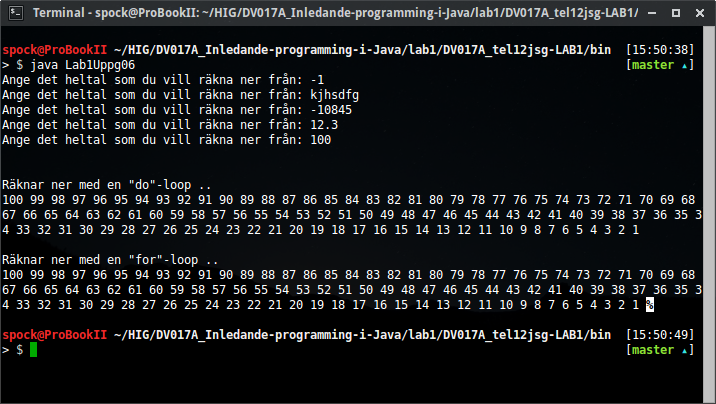
\includegraphics[width=\linewidth]{img/06.png}
    \caption{Körning av koden till Uppgift \ref{uppgift-6}}
    \label{fig:screenshot-06}
\end{figure}
